\documentclass{article}

\usepackage{swiftnav}
\usepackage{pgfplots}
\usepackage{filecontents}


\usepackage{subcaption}

\usepackage{draftwatermark, array}
\SetWatermarkLightness{0.9}
\SetWatermarkText{Preliminary}
\SetWatermarkScale{1}
% Suppress numbers from section headings (but preserve PDF TOC).
\makeatletter
\renewcommand\@seccntformat[1]{}
\makeatother
\newcolumntype{$}{>{\global\let\currentrowstyle\relax}}
\newcolumntype{^}{>{\currentrowstyle}}
\newcommand{\rowstyle}[1]{\gdef\currentrowstyle{#1}%
  #1\ignorespaces
}
\newenvironment{mpar}{\par\noindent\minipage{\linewidth}}{\endminipage\par}
%\setlength{\skip\mpfootins}{2cm}
\renewcommand{\thempfootnote}{(\arabic{mpfootnote})}


% ---------------------------------------------------------------------------
\usepackage[section]{placeins}
\version{0.1}
\title{Piksi for UAV Aerial surveying}
\mysubtitle{RTK direct georeferencing with Swift Navigation's Piksi GPS receiver}
\author{Dennis Zollo, Rai Gohalwar}
\date{\today}

\ignorespaces

\begin{document}
\maketitle

\thispagestyle{firstpage}

\section{Abstract}
\label{sec:abstract}
This whitepaper presents using Piksi, a Carrier Phase differential GPS sensor, to georeference aerial images from micro aerial vehicles (MAVs) for surveying use cases.
It presents both the sensor integration, data collection methods, and real world surveying results as processed by the PIX4D photogrammetry software.  Lastly, the value proposition of using RTK GPS for aerial surveying is evaluated.
\tableofcontents
\newpage
\section{Overview}
\label{sec:Overview}
Due to the capability, low-cost, and popularity of micro aerial vehicles, there is much interest about their potential applications including aerial surveying for industries such as precision agriculture, mining, and forestry.

In a typical aerial surveying use-case, an aircraft is outfitted with a high-quality camera and overflies an area of interest while capturing a series of images.  The images are then processed in software to produce Digital Elevation Models (DEM's), Orthomosaics, and/or 3D point clouds which can be used for photogrammetry applications, volumetric measurements, or crop health analysis to provide business value for users.

Commercial software tools for photogrammetry have the ability to stitch together aerial images through visual features with techniques such as Bundle adjustment.  These software packages often require rough location and orientation of the lense when the photo was taken.

To facilitate this post-processing, most low-cost MAV control systems used for photogrammetry have the ability to geotag photos as required by the processing software through Autonomous GPS combined with MEMS sensors.  The typical sensor technology, combined with uncertainty in timing of the camera's shutter, limits the precision and accuracy of geotagging information and requires post-processing software to rely heavily on image processing techniques. Additionally, large amounts of sidelap and overlap between images and ground control points are often required to allow post-processing software to utilize imagery information given the inaccuracy of the georeferencing information.  Lastly, survey sites lacking in visual detail (such as agricultural land) or where overlap is minimal (such as corridor mapping), often yield poor results with traditional techniques and sensors.

It has been demonstrated that Carrier Phase Differential GPS (also called Real Time Kinematic (RTK) GPS), can improve the location accuracy of georeferencing \cite{sensefly2}.  In the sections that follow, we will demonstrate methods and results of using Swift Navigation's Piksi GPS Receiver to geotag aerial photos for aerial surveying.  It is expected that precise and accurate geotagging information can reduce the need for ground control points for typical survey missions, reduce the amount of overlap and sidelap required, and improve the quality of ultimate photogrammetry deliverables.

\section{Equipment and Setup}
\label{sec:equipment}
\begin{figure}[h]
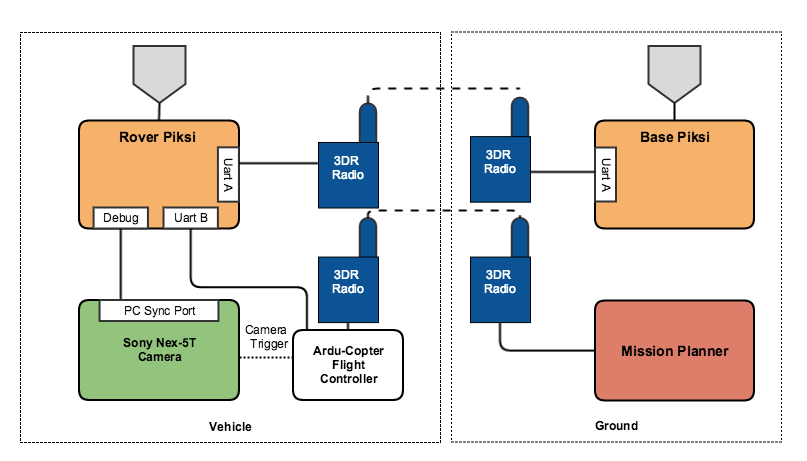
\includegraphics[width=7in]{images/flow_charts/uav_piksi_flow_chart.png}
\caption{Vehicle Diagram}
\label{figure:vehicle-diagram}
\end{figure}

\label{sec:equipment}
A camera, vehicle, and an image-tagging system using Piksi were developed to conduct experiments with careful design considerations.  Available and low cost COTS equipment was chosen to highlight that these results can be replicated without exotic or expensive equipment.  The camera chosen was a Sony NEX-5t with a fixed 20mm lense and a 16 MP CCID sensor.  The application required the ability to electrically sense the shutter which was achieved through the use of a "Fotasy SANEX Hot Shoe Adapter" Prontor/Compur (PC) socket for external flash Synchronization.  See table \ref{cameraspecs} for detailed camera specifications.

The vehicle was designed and sized to carry the camera payload for a typical surveying mission.  While a fixed wing aircraft may be more applicable to surveying missions for their increased range, a quadrotor configuration was chosen for low-cost and ease of implementation.  The test vehicle is based on a 680 Tarot quad frame and uses four TigerMotor antigravity 4006 motors with 15 inch propellers. The Pixhawk autopilot controls the aircraft and a 10.4Ah 6S battery pack powers. Fully loaded the copter has a flight time of about 30 minutes. The Sony camera is attached pointing down via a custom designed 3D printed a housing. Communication to both a base station Piksi and a UAV Ground control station was accomplished via two 3D Robotics point to point radio modems. See table \ref{table:vehicle-specs} for more information.
\begin{table}[]
\centering
\begin{tabular}{l^l}
\hline
\rowstyle{\bfseries}
Specification & Value \\ \hline
\rowstyle{}
Frame Type            & Quad-Rotor           \\ \hline
Frame                 & Tarot FY650          \\ \hline
Flight Controller     & 3DR Pixhawk          \\ \hline
Motors x 4            & T-Motor MN4006       \\ \hline
Motor Controllers x 4 & X-Rotor 40A OPTO     \\ \hline
Propellers x 4        & Tarot 1555 CF        \\ \hline
Batteries x 2         & Multistar 6S 5200mAh \\ \hline
Weight                & 2942 g               \\ \hline
\end{tabular}
\caption{Vehicle Specifications}
\label{table:vehicle-specs}
\end{table}

\begin{table}[]
\centering
\begin{tabular}{|l|c|}
\hline
\multicolumn{2}{|c|}{GPS Specifications} \\ \hline
Primary GPS         & Piksi v2.3.1       \\ \hline
Secondary GPS       & U-Blox NEO 7N      \\ \hline
Primary Antenna     & Tellysman TW2412   \\ \hline
Secondary Antenna   & Taoglas gp.1575    \\ \hline
\end{tabular}
\label{table:gps}
\caption{Vehicle GPS Specifications}
\end{table}

\section{Method}
\label{sec:method}
Site selection
GCP surveying (skylark)
Mission Planning (mission planner)
Camera setup (exposure, etc)

\begin{table}[]
\centering
\begin{tabular}{l ^ l}
\hline
\rowstyle{\bfseries}
Specification & Value \\ \hline
\rowstyle{}
Camera                                                                & Sony Nex-5T        \\ \hline
Lens                                                                  & Sony SEL-20F28 (20mm)     \\ \hline
\begin{tabular}[c]{@{}l@{}}Weight\\ (with vehicle mount)\end{tabular} & 424 g              \\ \hline
Sensor                                                                & 16 MP: 4912 x 3264 \\ \hline
Hot shoe adapter \begin{tabular}[c]{@{}l@{}}Fotasy SANEX Hot Shoe Adapter \\(ASIN: B00DE4T4E2)\end{tabular}  \\ \hline
\end{tabular}
\caption{Camera Specifications}
\label{cameraspecs}
\end{table}

%add info about how we collected the data for the GCP's

When conducting a surveying mission, it is very important to configure the vehicle, camera, and flight parameters. To set flight parameters and other surveying parameters, Mission Planner GCS was used. Mission Planner provided flight status during the mission and tools to convert user defined surveying parameters (ground sampling distance, overlap, sidelap, area of interest, flight time and camera direction) into an autonomous mission for Pixhawk.

The mission analyzed in this paper was designed with UAV surveying standards in mind. With a 75 percent overlap and 60 percent sidelap, the vehicle flew for approximately 22 minutes to capture 218 images. The copter in this mission was flown at 20m altitude which in theory gives a 2.37 mm GSD. Pix4D reported an average GSD of 4.9 mm due to the terrain change and altitude variations of the vehicle during the mission. Figure \ref{flightplan} shows the flight plan of the copter and the locations of the ground control points.

\begin{figure}
\begin{center}
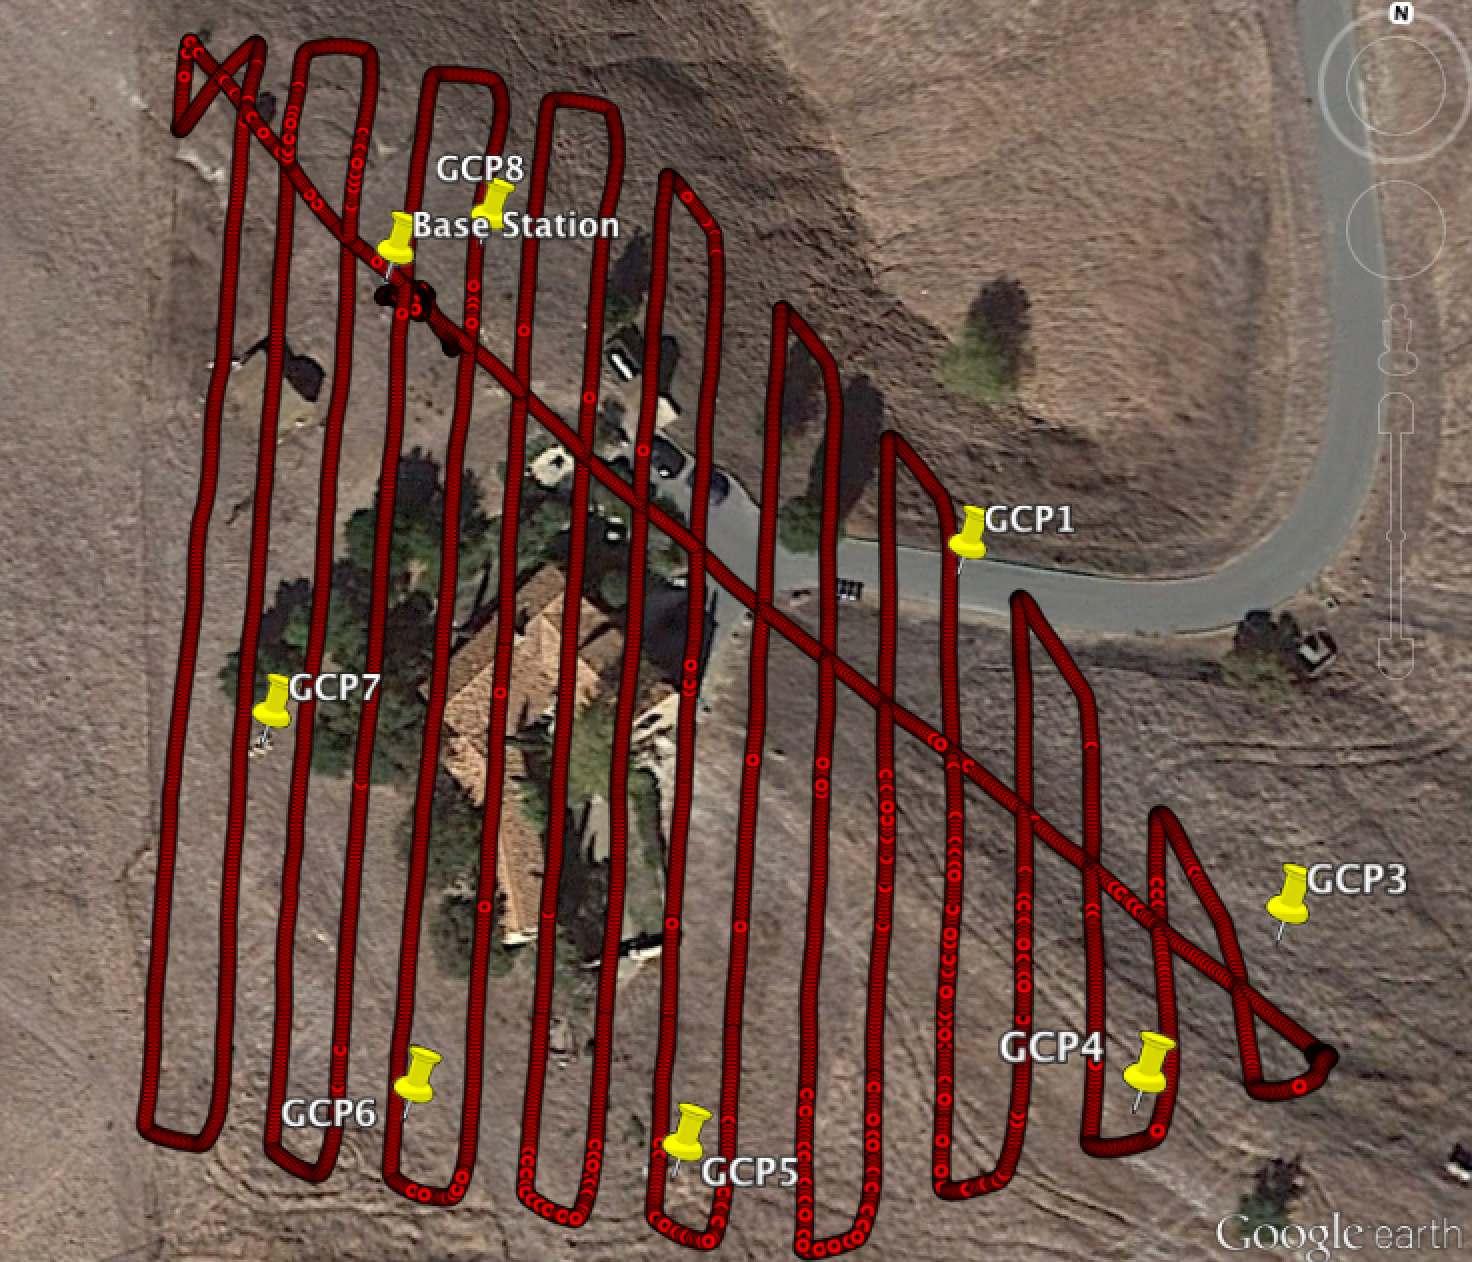
\includegraphics[width=5in]{images/flight_plan_gcp.png}
\caption{Flight plan visualization}
\label{flightplan}
\end{center}
\end{figure}

To get the best quality possible, it was also necessary to configure the camera settings appropriately. During some of the initial testing, many of the images were coming out blurry. In order to compensate for the continuous movement of the copter and the vibrations, a constant shutter speed of 1/1250 sec was selected. The aperture settings were auto selected by the camera. This resulted in sharp and detailed images.

\section{Post-Processing Techniques}
\label{sec:postprocessing}
Post processing tools were developed in house for this project. Images captures from the camera were not individually tagged. Instead , a file with the image names, Piksi geo-loacaiton data (WGS84) , orientation data (omega, phi, kappa) and accuracy (default of 5m horizontal and 10m vertical) was generated. This file was fed into Pix4D along with the images. Even though 7 GCPs (Ground Control Points) were measured, none were used in the processing.

Figure \ref{postprocess} shows the basic layout of the post-processing routines as to allow the methods to be reproduced.  Georeference-process.py is a top-level python script that processes the data and generates a .csv file with image Geolocations that can be consumed by Pix4d. There are other scripts within that carry out individual tasks. Mavlink-decode.py extracts the piksi log file (SBP JSON) from the dataflash BIN log file created by the Pixhawk. Interpolate-event.py linearly interpolates the position data at the trigger points using the SBP log file. Query-mavlink.py is used to extract the attitude data at each shutter time. This attitude data is converted from Euler angle centi-degrees to the surveying coordinate frame (omega/phi/kappa) in a subroutine in Georeference-process.py. All this data is then compiled into a csv file formate specified by Pix4d with a Geolocation and camera attitude for each image.  All scripts are open-source software available from Swift Navigation's Github repositories \url{http://github.com/swift-nav}

\section{Photogrammetry parameters}
In order to compare and analyze results from Pix4D, a total of 12 variations of settings and data were selected for rendering as described in table \ref{table:postparams}.  The Calibration method column refers to whether the "Standard" calibration method in Pix4d or the "Accurate Geolocation and Orientation" methods were used.  According to Pix4d help documentation, the "Accurate" setting is "Optimized for project with very accurate image geolocation and orientation. This calibration method requires all images to be geolocated and oriented."\cite{pix4d_support1}  The Included images column refers to which images were used for post-processing (see section \ref{sec:overlap} for more information)
The entire parameter space was repeated for the primary GPS (Piksi) and control GPS sensor (Ublox sensor).


\begin{figure}
\begin{center}
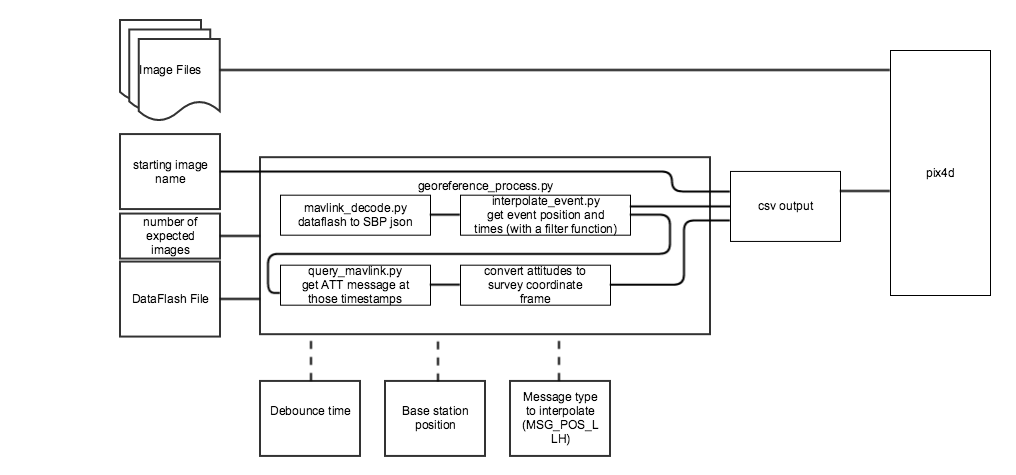
\includegraphics[width=7in]{images/flow_charts/uav_survey_processing_architecture.png}
\caption{Post Processing Architecture}
\label{postprocess}
\end{center}
\end{figure}

\begin{table}
\begin{tabular}{l ^ l ^ l ^ l ^ l ^ l} \\ \hline
\rowstyle{\bfseries}
Config & Description & Calibration Method & Included Images & GPS Sensor & Ground Control \\ \hline
\rowstyle{}
1  & Piksi RTK Std             & Standard  & All               & Piksi RTK (Fixed) & None \\ \hline
2  & Piksi RTK Std low sidelap & Standard  & Every Other Line  & Piksi RTK (Fixed) & None   \\ \hline
3  & Piksi RTK Std low overlap & Standard  & Every Other Image & Piksi RTK (Fixed) & None  \\ \hline
4  & Piksi RTK Std GCP         & Accurate  & All               & Piksi RTK (Fixed) & 7 GCPs \\ \hline
5  & Piksi RTK Acc             & Accurate  & All Images        & Piksi RTK (Fixed) & Nonoe \\ \hline
6  & Piksi RTK Acc GCP         & Accurate  & All               & Piksi RTK (Fixed) & 7 GCPs \\ \hline
7  & Ublox Std                 & Standard  & All               & Ublox             & None   \\ \hline
8  & Ublox Std low sidelap     & Standard  & Every Other Line  & Ublox             & None \\ \hline
9  & Ublox Std low overlap     & Standard  & Every Other Image & Ublox             & None  \\ \hline
10 & Ublox Std GCP             & Standard  & All               & Ublox             & 7 GCPs \\ \hline
11 & Ublox Acc                 & Accurate  & All               & Ublox             & None \\ \hline
12 & Ublox Acc GCP             & Accurate  & All               & Ublox             & 7 GCPs \\ \hline
\end{tabular}
\caption{Post processing parameterization}
\label{table:postparams}
\end{table}


\begin{figure}
\centering
\renewcommand*\thesubfigure{\arabic{subfigure}}
\begin{subfigure}{.33\textwidth}
  \centering
  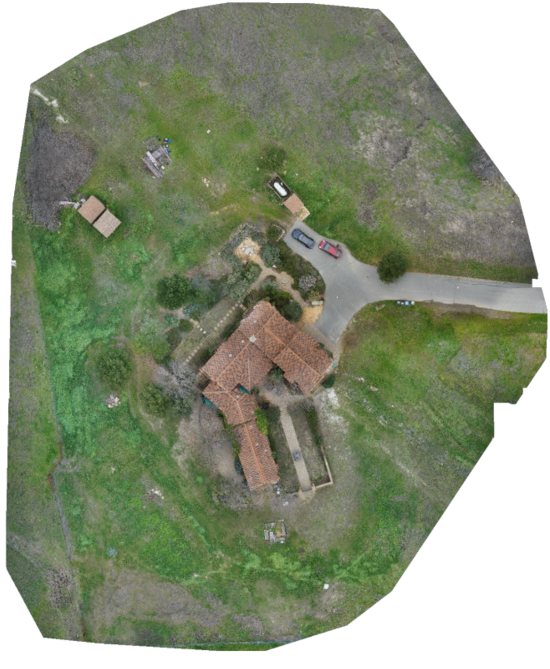
\includegraphics[width=.75\linewidth]{images/orthomosaics/p.png}
  \caption{Piksi all images}
  \label{fig:sub1}
\end{subfigure}%
\begin{subfigure}{.33\textwidth}
  \centering
  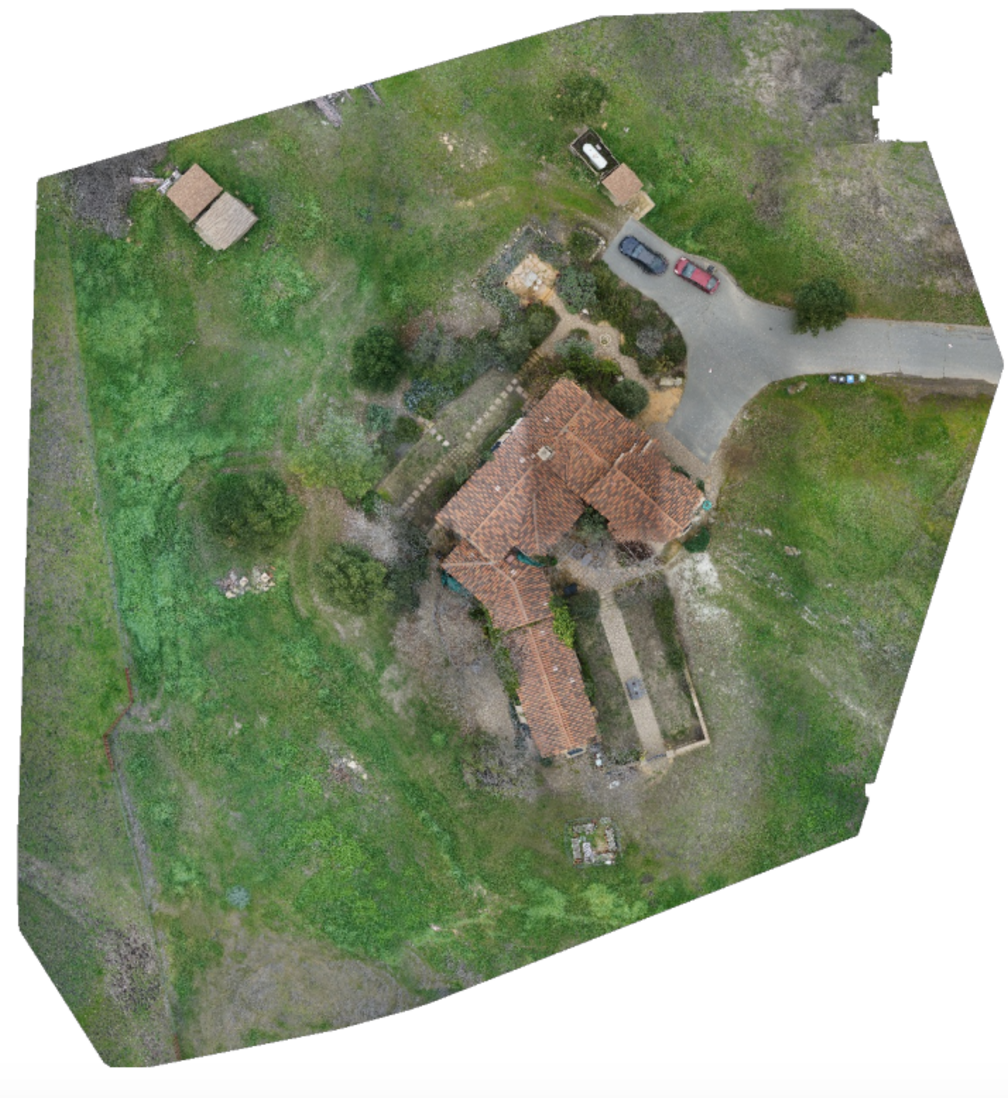
\includegraphics[width=.75\linewidth]{images/orthomosaics/p_every_other_line.png}
  \caption{Piksi every other line}
  \label{fig:sub2}
\end{subfigure}
\begin{subfigure}{.33\textwidth}
  \centering
  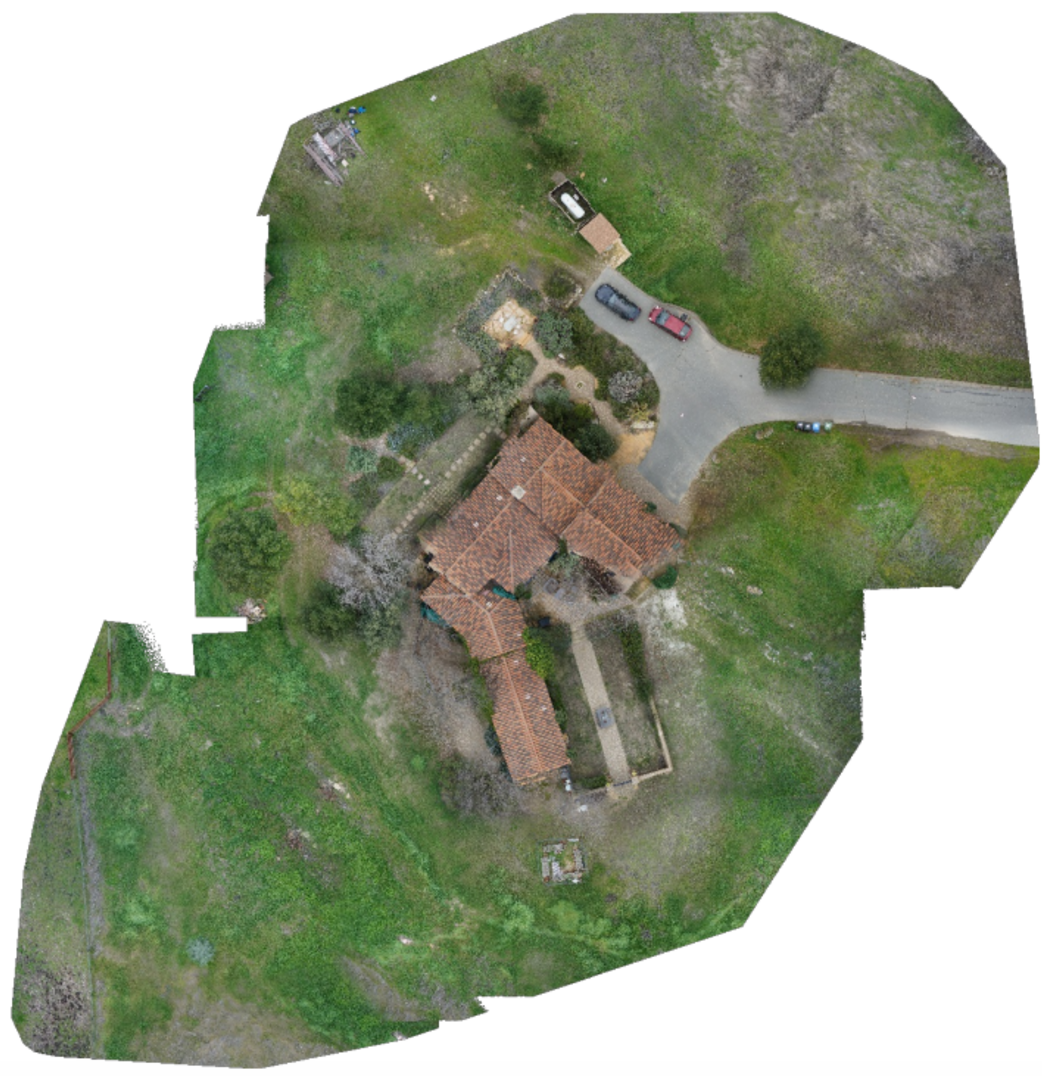
\includegraphics[width=.75\linewidth]{images/orthomosaics/p_every_other_image.png}
  \caption{Piksi Every Other Image}
  \label{fig:sub1}
\end{subfigure}%
\begin{subfigure}{.33\textwidth}
  \centering
  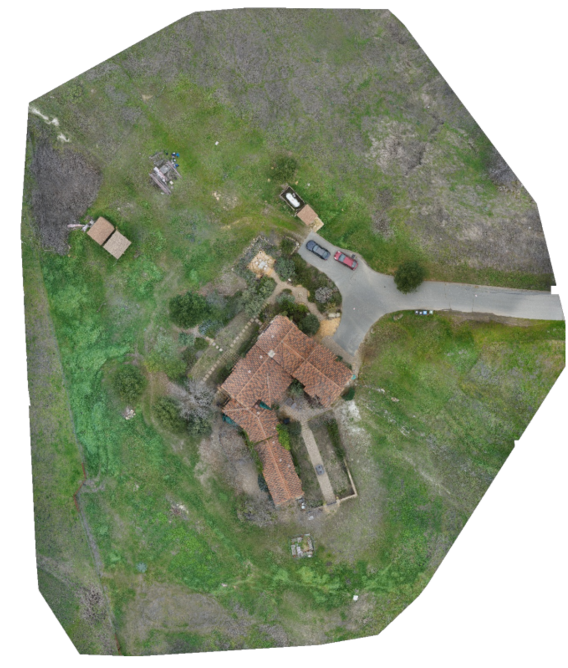
\includegraphics[width=.75\linewidth]{images/orthomosaics/p_gcp.png}
  \caption{Piksi with GCPs}
  \label{fig:sub1}
\end{subfigure}%
\begin{subfigure}{.33\textwidth}
  \centering
  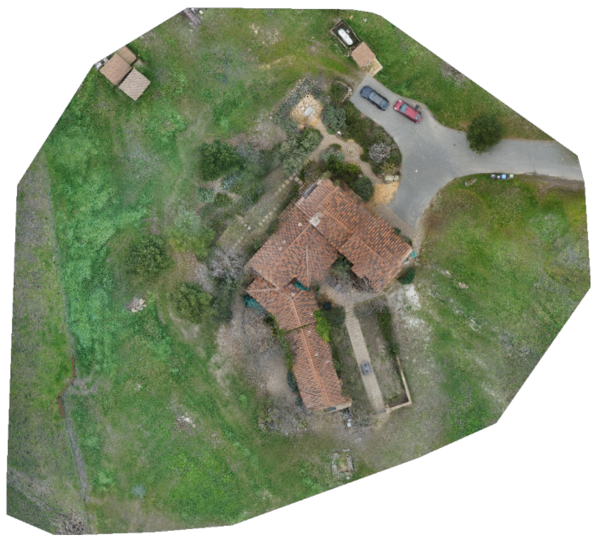
\includegraphics[width=.75\linewidth]{images/orthomosaics/p_accurate.png}
  \caption{Piksi Accuracy }
  \label{fig:sub2}
\end{subfigure}
\begin{subfigure}{.33\textwidth}
  \centering
  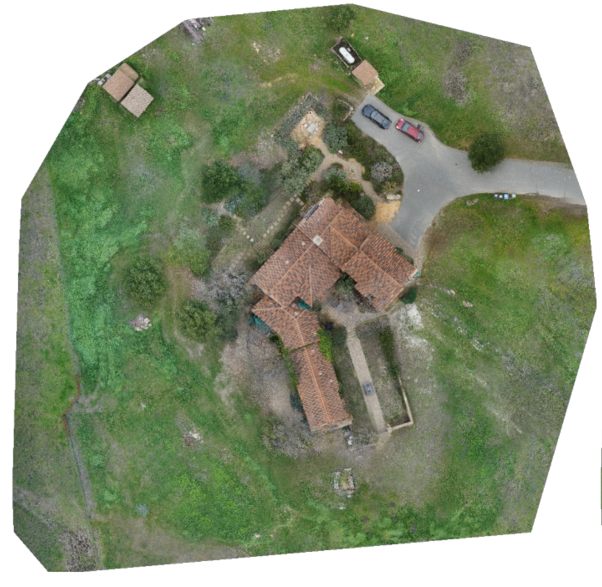
\includegraphics[width=.75\linewidth]{images/orthomosaics/p_gcp_accurate.png}
  \caption{Piksi Accuracy with GCPs}
  \label{fig:sub1}
\end{subfigure}%
\begin{subfigure}{.33\textwidth}
  \centering
  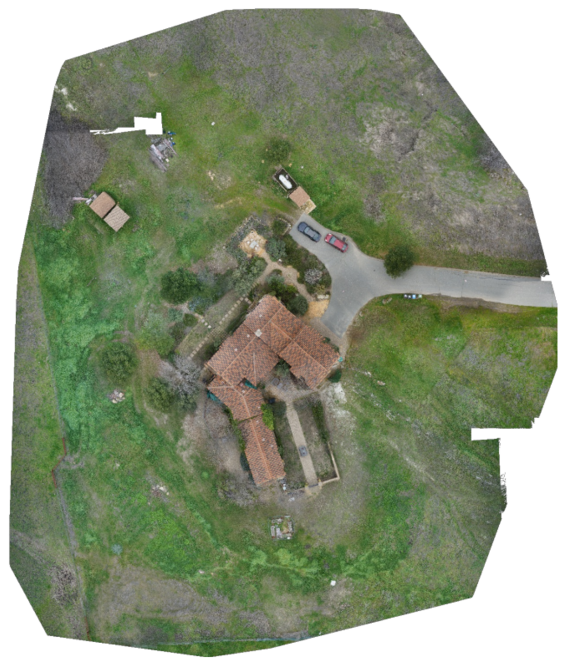
\includegraphics[width=.75\linewidth]{images/orthomosaics/ublox.png}
  \caption{Ublox All Images}
  \label{fig:sub1}
\end{subfigure}%
\begin{subfigure}{.33\textwidth}
  \centering
  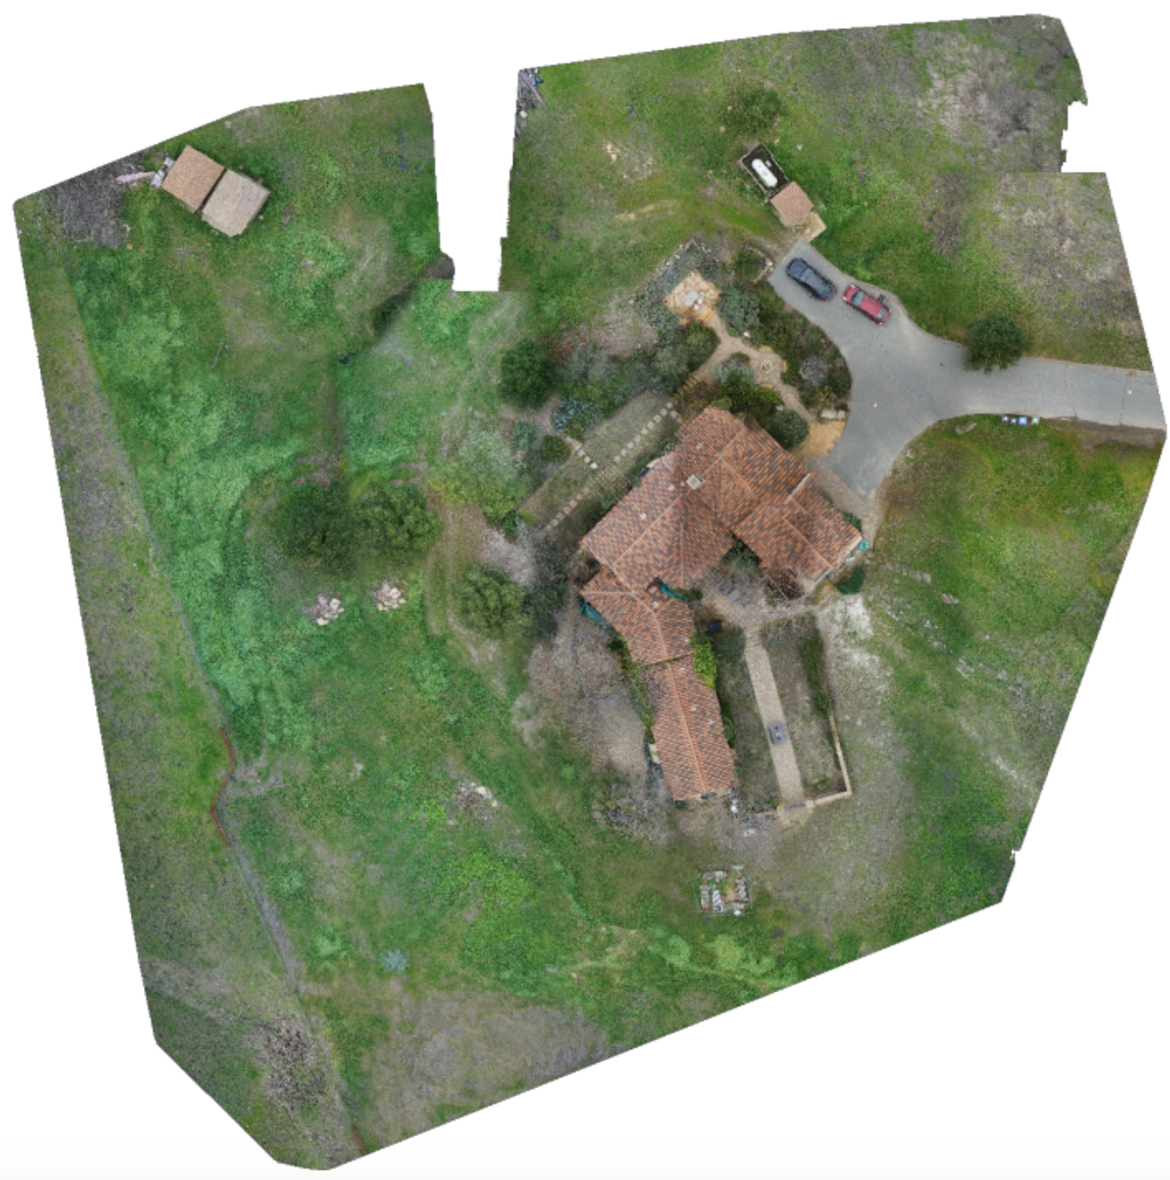
\includegraphics[width=.75\linewidth]{images/orthomosaics/ublox_every_other_line.png}
  \caption{Ublox Every Other Line}
  \label{fig:sub2}
\end{subfigure}
\begin{subfigure}{.33\textwidth}
  \centering
  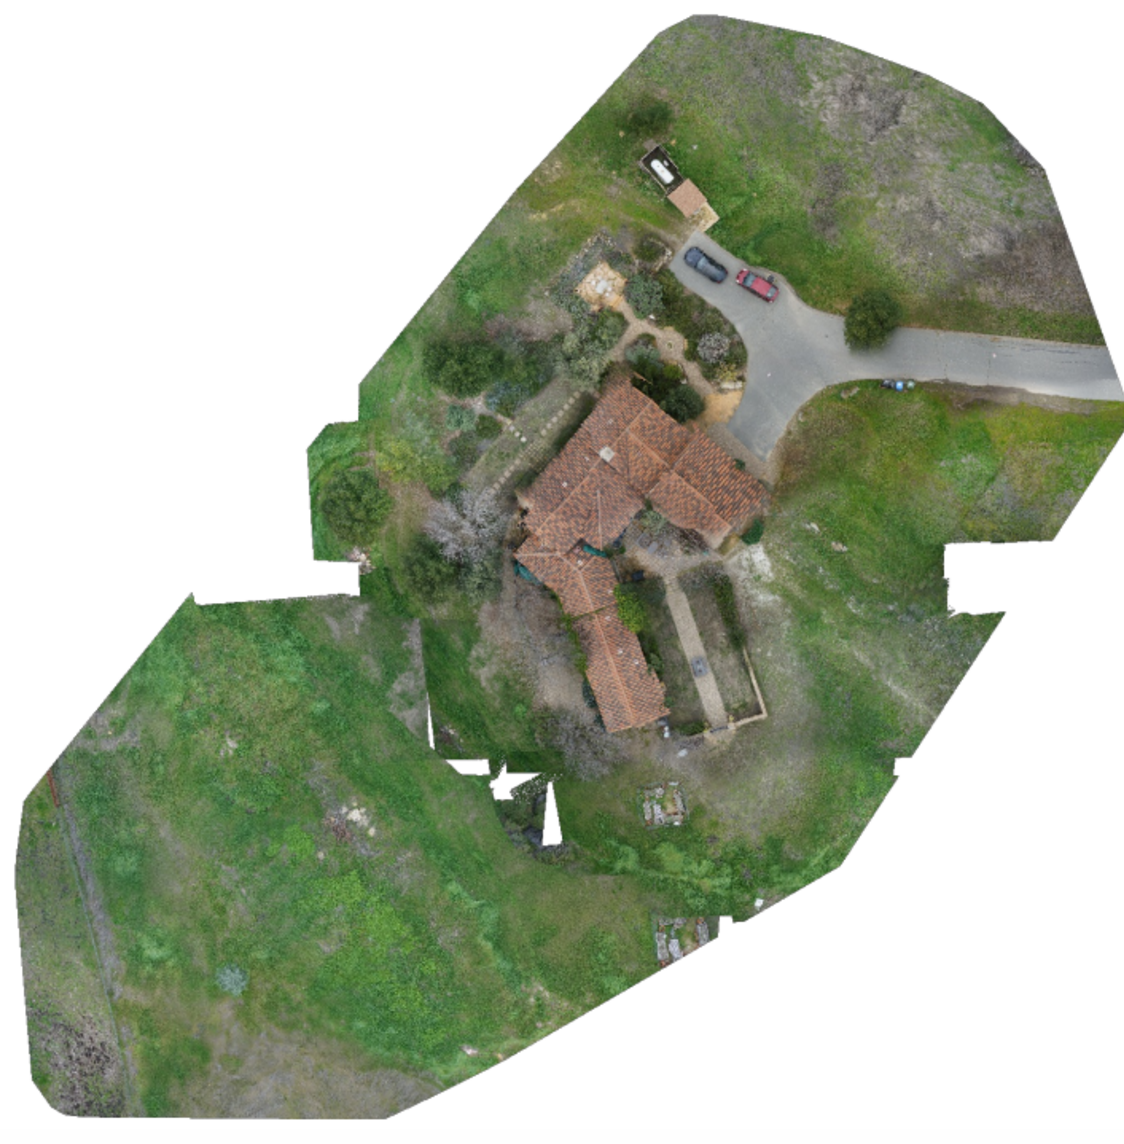
\includegraphics[width=.75\linewidth]{images/orthomosaics/ublox_every_other_image.png}
  \caption{Ublox Every Other Image}
  \label{fig:sub1}
\end{subfigure}%
\begin{subfigure}{.33\textwidth}
  \centering
  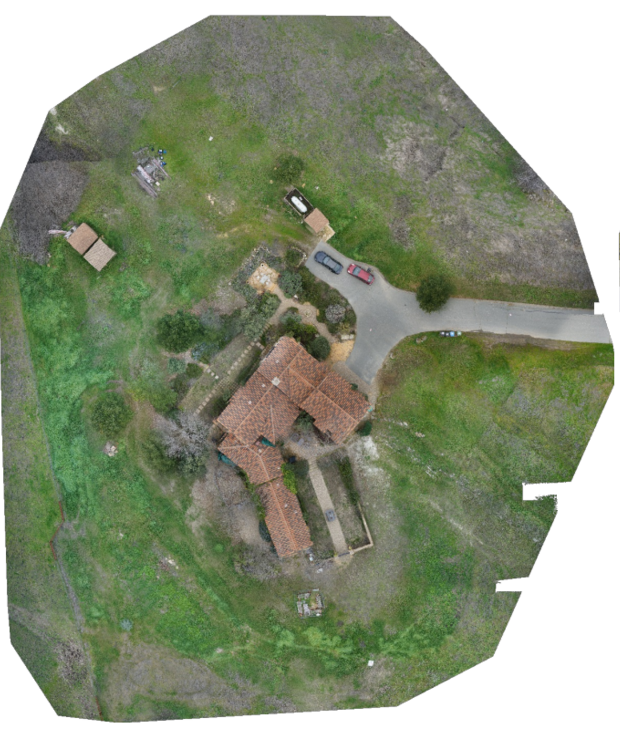
\includegraphics[width=.75\linewidth]{images/orthomosaics/ublox_gcp.png}
  \caption{Ublox with GCPs}
  \label{fig:sub1}
\end{subfigure}%
\end{figure}

\section{Results: Accuracy}
talk about accuracy of each method

Accuracy is very important when conducting a surveying mission. Ideally GCPs help post-procesing softwares refine the scale and help align the images better. Without GCPs , Pix4D would have a hard time computing the true scale of the image unless the geo-tags were really accurate. In order to test the accuracy of Piksi , we setup a test where we used Pix4D to measure the distance between 2 GCP markers. As shown in Figure ?? , these markers were red and white. Before the mission we collected the locations of these markers very accurately. Using some post-processing tools, we compared the calculated distances to the measured distance of 54.83 metres. There was little to no difference between the distance Piksi renderings showed compared to the ublox renderings. The hypothesis is that, if the data is within a threshold, Pix4D considers the geolocation data minutely. Most of the stitching and scaling is done from image processing.

In pursuite of finding a way to give more significance to the geolocation data, [andrew scited] from PixD suggested using the "Accurate Geolocation and Orientation" setting. Found in the settings section, this parameter allows Pix4D to rely more on the geolocation and orientation data provided by the user.

Configuration 5, 6, 11 and 12 were rendered using "Accurate Geoloaction and Orientation" settings in Pix4D. One would think that using this setting would produce better results; however the results say otherwise. Observing table ?? , both Piksi and Ublox suffer from this setting. The RMS errors increase to a point that configuration 11 doesn't produce DSM or otrhomosaic and configuration 12 doesn't render at all. In Figure ?? the orthomosaics of Piksi clearly show the inaccuracy of renders with this setting compared to default settings. The mosaic of configuration 5 is literally half the area compared to configuration 1.

The only theory that explains this behavior is the orientation data. Since the Pixhawk flight controller have a mems IMU, it brings about a lot of error in the orientation. Moreover the conversion in Pix4D from centidegrees to omega/phi/kappa is questionable. Therefor the only logical source of error is bad orientation data which Pix4D heavily relies upon. Unfortunately there is no known way to ONLY use the geolocation data. Therefor, this effort to improve accuracy was dropped.

\begin{tabular}{l ^ l ^ l ^ l ^ l} \hline
\rowstyle{\bfseries}
Configuration & X Error [m] & Y Error [m] & Z Error [m] & Image calibrated [percent]   \\ \hline
\rowstyle{}
1 & 0.185 & 0.136 & 0.274 & 84   \\ \hline
2 & 0.653 & 0.552 & 1.056 & 64    \\ \hline
3 & 0.847 & 1.182 & 1.202 & 59  \\ \hline
4 & 0.076 & 0.089 & 0.011 & 85    \\ \hline
5 & 0.556 & 0.619 & 0.989 & 99  \\ \hline
6 & 0.277 & 0.073 & 0.723 & 95   \\ \hline
7 & 0.202 & 0.840 & 0.563 & 82   \\ \hline
8 & 3.075 & 1.842 & 1.255 & 64   \\ \hline
9 & 2.191 & 3.028 & 1.897 & 57  \\ \hline
10 & 0.086 & 0.096 & 0.024 & 81   \\ \hline
11 & 0.500 & 0.625 & 0.959 & 99   \\ \hline
12 & WOULD & NOT & RENDER   \\ \hline
\end{tabular}




\section{Results: Overlap/Sidelap}
\label{sec:overlap}
Currently, surveying missions are flown with 70 to 80 percent overlap to get decent results from their data. The purpose of this high overlap is so that the user can collect plenty of data for the post-processing tools. Tools such as Pix4D are designed to favor image processing over geolocation information due to lack of accuracy in the commonly used GNSS systems on micro UAVs. The hypothesis
is that with accurate geolocation data, the overlap percentage can be dropped without effecting the performance.

The mission was designed to have an overlap of 75 percent and a side lap of 60 percent. The idea behind these numbers was so that in post processing we could eliminate lines and images and still be able to process the data. Figure ?? shows the errors extracted from Pix4D quality reports for various configurations. Both Piksi and Ublox experience significance increase in error when lines and images are removed. That being said, the magnitude of Piksi's error is magnitudes smaller than of Ublox.


\begin{figure}
\centering
\begin{subfigure}{.5\textwidth}
  \centering
  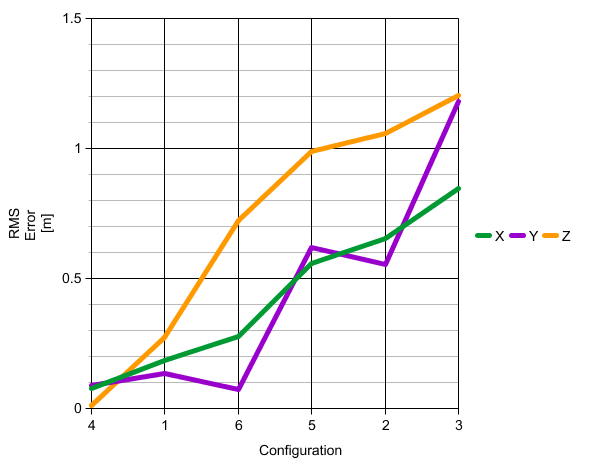
\includegraphics[width=1\linewidth]{images/piksi_rms_error.png}
  \caption{Piksi}
  \label{fig:sub1}
\end{subfigure}%
\begin{subfigure}{.5\textwidth}
  \centering
  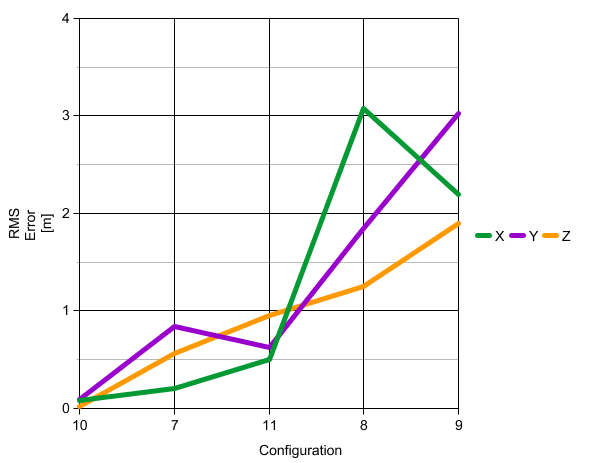
\includegraphics[width=1\linewidth]{images/ublox_rms_error.png}
  \caption{Ublox}
  \label{fig:sub2}
\end{subfigure}%
\end{figure}

\section{Results: Initial accuracy estimate investigation}
One potential output to measure post-processing quality is the RMS errors reported by Pix4d Software which come from the "Initial processing" step of the software.  Indeed, the marketing material of some vendors and other parts of the literature use this image processing output as a key metric in evaluating the quality of geolocation surveying data.

In this analysis, however, the RMS errors values seemed highly affected by the image geolocation "accuracy" estimates are initially provided to the software by the user as input.  This outcome was peculiar and unexplained.  This odd relationship is presented in table [TABLE HERE]. The table shows three identical post-processing runs where the only difference was the accuracy estimate.  As this accuracy estimate decreased, the image location errors as reported in the Pix4d quality report decreased as well.  This behavior suggests that the accuracy reported by Pix4d for geolocation information is more an artifact of post-processing than representing something physical. As an additional note, in certain cases when these initial accuracy values are constrained to values below the accuracy of the sensors used for geo-referenceing, the software is unable to perform initial processing.
 % images processed  2d keypoints mean RMS Error [m] X RMS Error [m] Y RMS Error [m] Z

\begin{tabular}{l ^ c ^ c ^ l ^ l ^c ^c ^c} \hline
\rowstyle{\bfseries}
Label & \multicolumn{2}{^c}{Initial Image Accuracy [m]}  & Images & 2d keypoints & \multicolumn{3}{^c}{Mean RMS Error [m]} \\
&   X,Y & Z & processed (\%) & & X & Y & Z  \\ \hline
\rowstyle{}
a  &5   &10  &84  &5902  &0.184857  &0.136434  &0.273608 \\ \hline
b  &0.2 &1   &84  &5907  &0.126739  &0.097678  &0.163582 \\ \hline
c  &0.1 &0.2 &84  &5887  &0.061538  &0.06066   &0.111367 \\ \hline
\end{tabular}

\begin{thebibliography}{9}
\bibitem{sensefly1}
Strechha,  Christophe (2011). \textit{The Accuracy of Automatic Photogrammetric Techniques on Ultra-Light UAV Imagery}. UAV-g 2011 - Unmanned Aerial Vehicle in Geomatics, Zürich, CH, September 14-16, 2011
\bibitem{sensefly2}
A. Roze, J-C. Zufferey, A. Beyeler, A. McClellan \textit{eBee RTK Accuracy Assessment}.
Retrieved from \url{https://www.sensefly.com/fileadmin/user_upload/sensefly/documents/eBee-RTK-Accuracy-Assessment.pdf}

\bibitem{pix4d_support1}
"Menu Process Processing Options... 1. Initial Processing Calibration." Pix4d. Retrieved March 24, 2016, from https://support.pix4d.com/hc/en-us/articles/205327965#label2&gsc.tab=0
\end{thebibliography}
\thispagestyle{lastpage}
\end{document}
